
\section{Seismicity Parameters}

For each of the three seismic regions, Gutenberg-Richter parameters and maximum magnitude ($M_{max}$) were calculated using Seismic Hazard Assessment code (HA3) \citep{kijko2004}. The regional maximum magnitude for each region is estimated by the \citet{Kijko1989} method, which is implemented in the HA3 package. For smoothed seismicity areas, $b-value$ is assumed constant. The $a-value$ can vary spatially and is determined by counting earthquakes above $M$ 3.0 in each grid cells.

\citet{Karimiparidari2013} applied the Maximum Curvature (MAXC) technique \citep{Wyss1999, Wiemer2000} by ZMap \citep{Wiemer2001} to calculate the level of completeness of instrumental part of the catalog.  Following the \citet{Karimiparidari2013}, we assume the catalog is complete for earthquakes with magnitude 4.5, 4.4, 4.5, 4.5, and 4.4 for Azerbaijan, Alborz,  Kopeh-Dagh, Central Iran, and Zagros tectonic seismic regions, respectively. For the uniform model we used 4.5 as a completeness magnitude. In this study we use those magnitudes of completeness as the magnitude threshold in the calculation of the seismicity parameters. We also used the seismicity parameters of \citet{Karimiparidari2013} as the priory information in HA3 code. The updated values are displayed in Table \ref{tab:b_value}.  Annual occurrence rate of the earthquake for each region is shown in Fig.~\ref{fig:annual_m}.

\begin{figure*}[t]
    \centering
    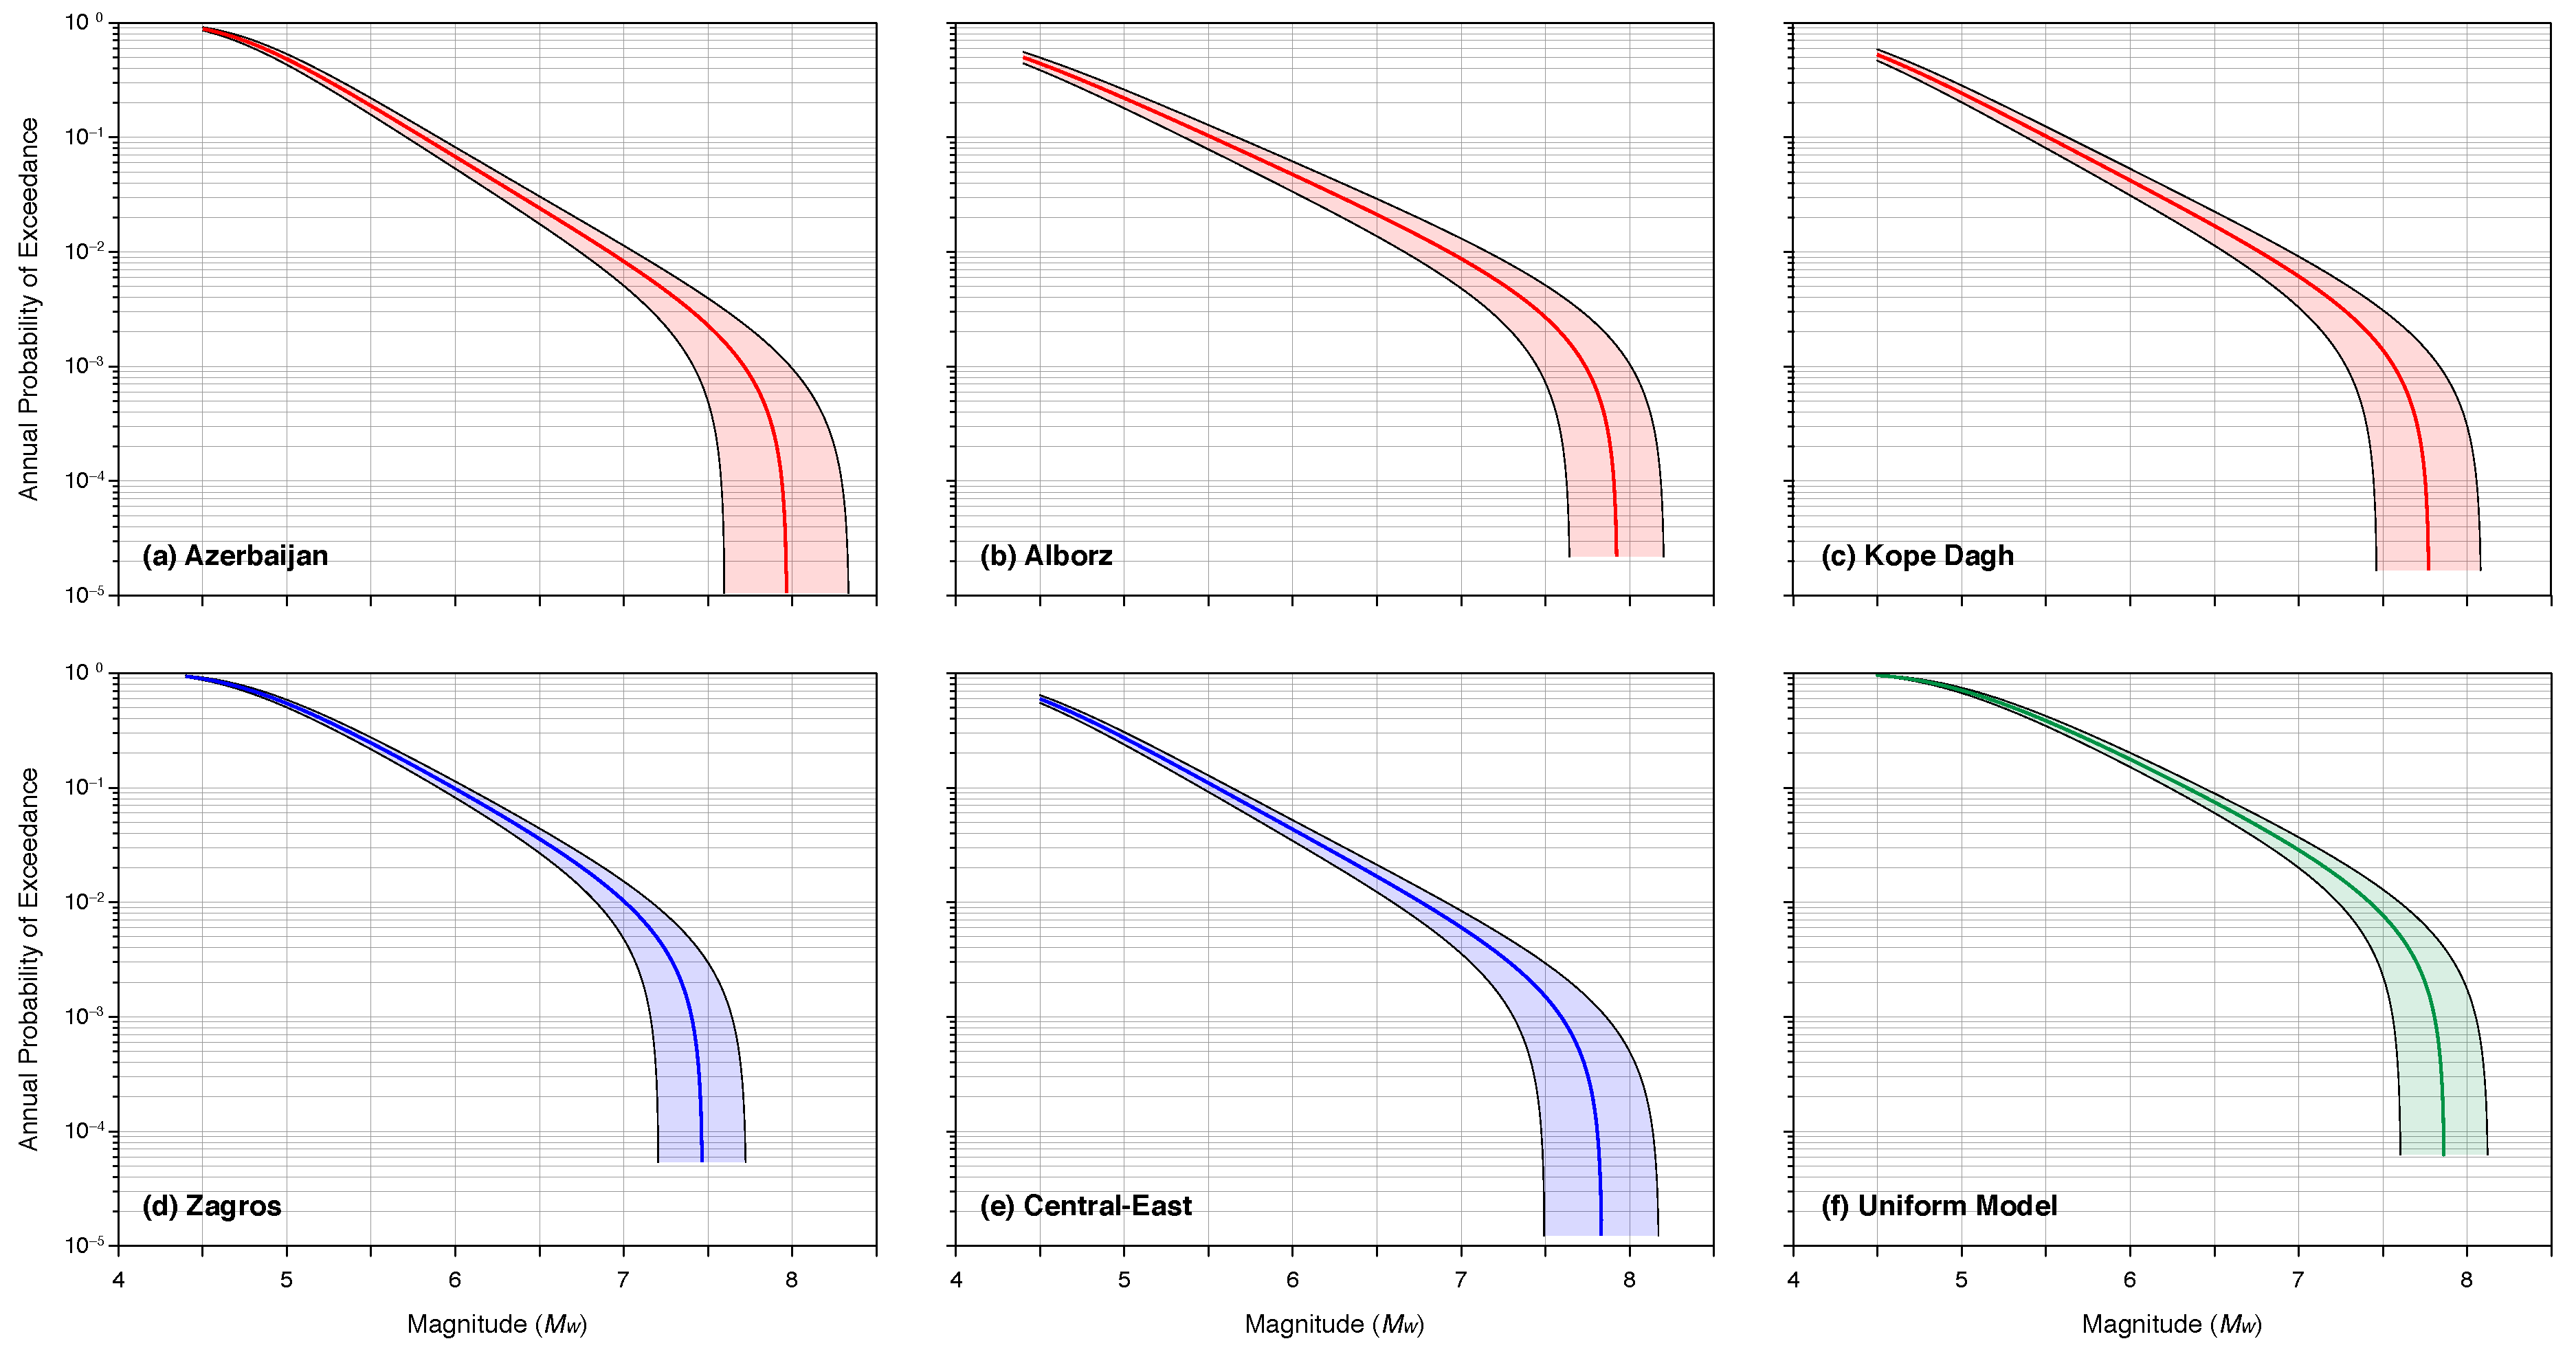
\includegraphics[width=\textwidth]{figures/pdf/figure-04} 
    \caption{Annual probability of exceedance as a function of earthquake magnitude for seismic tectonic regions of (a) Alborz, (b) Azerbaijan, (c) Central Iran, (d) Kopeh Dagh, (e) Uniform (f) Zagros. The shaded range indicates the models' $\pm 1$ standard deviation.}
    \label{fig:annual_m}
\end{figure*}

\begin{table*}[t]
    \centering
    \caption{Seismicity parameters for the tectonic seismic regions influencing seismic hazard in northern Iran.}
    \begin{tabular}{ccccc}
        \hline                                                                              \\[-1.6ex]
                        & $b$-value         & Computed $M_{\max}$   & Observed $M_{\max}$   \\[0.6ex]
        \hline                                                                              \\[-1.6ex]
        Azerbaijan      & 1.10 $\pm$ 0.03   & 7.93 $\pm$ 0.34       & 7.7                   \\
        Alborz          & 1.03 $\pm$ 0.03   & 7.85 $\pm$ 0.66       & 7.8                   \\
        Kopeh Dagh      & 0.89 $\pm$ 0.04   & 7.78 $\pm$ 0.31       & 7.6                   \\
        Zagros          & 0.99 $\pm$ 0.02   & 7.47 $\pm$ 0.26       & 7.4                   \\
        Central-East    & 0.95 $\pm$ 0.04   & 7.84 $\pm$ 0.34       & 7.6                   \\
        Uniform Model   & 0.90 $\pm$ 0.02   & 7.87 $\pm$ 0.26       & 7.8                   \\[0.5ex]
        \hline 
    \end{tabular}
    \label{tab:b_value} 
\end{table*}

